\section{The Design of TD-Pipe}

\begin{figure*}[htbp]
    \centering    
\includegraphics[width=0.95\linewidth]{fig/overview.pdf}
    \caption{The system overview of TD-Pipe.}
    \label{fig:overview}
\end{figure*}


The key idea of TD-Pipe lies in the temporally-disaggregated pipeline parallelism architecture which disaggregates the prefill and decode phases in the temporal dimension.
Basically, TD-Pipe aims to achieve high-throughput offline LLM inference in the multi-GPU architecture, particularly on commodity nodes without GPU-direct interconnection cables.
Figure~\ref{fig:overview} demonstrates the overall design of TD-Pipe.
At first, TD-Pipe follows a hierarchy-controller structure, which abstracts the system into a centralized engine and a distributed runtime, responsible for controlling and execution respectively. 
Through decoupling the scheduling from execution, it can coordinate multiple devices in a pipeline asynchronously.

Next, TD-Pipe identifies three fundamental requirements in the temporally-disaggregated pipeline parallelism architecture and addresses them by three novel approaches.
First, the AI-based greedy prefill approach aggressively delays and determines the timing for switching from prefill to decode.
It performs more prefills within a fixed memory capacity by predicting output lengths and calculating the optimal point.
Second, the inter-batch work stealing approach reduces pipeline bubbles caused by random request completion in different batches and dynamically redistributes workloads from heavy to light batches.
Third, the spatial-temporal intensity comparison approach  determines the timing for switching from decode to prefill by comparing the performance cost between the reduced computational intensity and the pipeline bubbles caused by switching.
Finally, TD-Pipe achieves compact pipeline scheduling with very minimal bubbles in phase switching.


\subsection{Temporally-Disaggregated Pipeline}

As stated in Section \S \ref{sec:batching}, naively integrating separate batching into pipeline parallelism leads to severe bubble issues, primarily due to data dependencies and workload imbalance.
To address this, we adopt a temporal disaggregation strategy that separates the prefill and decode phases in the temporal dimension, thereby minimizing their mutual interference.
In this design, each inference instance processes only a single phase type over a long period of time, significantly reducing pipeline bubbles.
The prefill phase and the decode phase operate in a producer-consumer relationship, where the decode phase relies on the completion of the prefill phase.
Consequently, phase switching remains necessary.
To further improve this architecture, we aim to reduce the frequency of phase switching while maintaining high efficiency within each phase.


\subsection{Hierarchy-controller System Structure}

To make devices collaborate better, we design the hierarchy-controller system structure for TD-Pipe.
To handle the complex data dependencies and enable asynchronous data transmission simultaneously, as shown in Figure~\ref{fig:overview}, it decouples the scheduling and execution of pipeline tasks, abstracting the centralized engine as the control plane and the distributed runtime as the execution plane.
The centralized engine is responsible for batch scheduling based on memory capacity, request status, and profiling results, and then launching tasks to workers of distributed runtime.
The distributed runtime is responsible for detailed execution and each worker only knows what data and which device it should communicate.

\subsubsection{Centralized Engine}
The centralized engine manages and controls workers via remote procedure call (RPC).
It is primarily responsible for two distinct stages, i.e. runtime initialization and execution scheduling.
During initialization, it delegates sub-models to workers, initializes the relevant parts of the model and loads parameters into memory.
Execution scheduling deals with batching requests and sending control information to workers.
For the prefill phase, the engine packs prompts and directly sends them to workers until the switching condition is triggered.
For the decode phase, the engine packs decode steps as batches and is also responsible for deleting these completed requests at each iteration.

\subsubsection{Distributed Runtime}

As only the execution plane, the distributed runtime follows the idea of the single program multiple data (SPMD) model, that each worker only knows what data it should compute, what data it should communicate, and which device it should communicate to.
To manage the communication meta-information, such as world size and rank number, a global communication context is initialized.
In this way, after receiving information distributed by the centralized engine, a worker knows its position based on the global communication context, and it can perform the point-to-point communication between pipeline stages asynchronously.

\subsection{Approach-1: AI-based Greedy Prefill}

\begin{figure}[!t]
    \centering    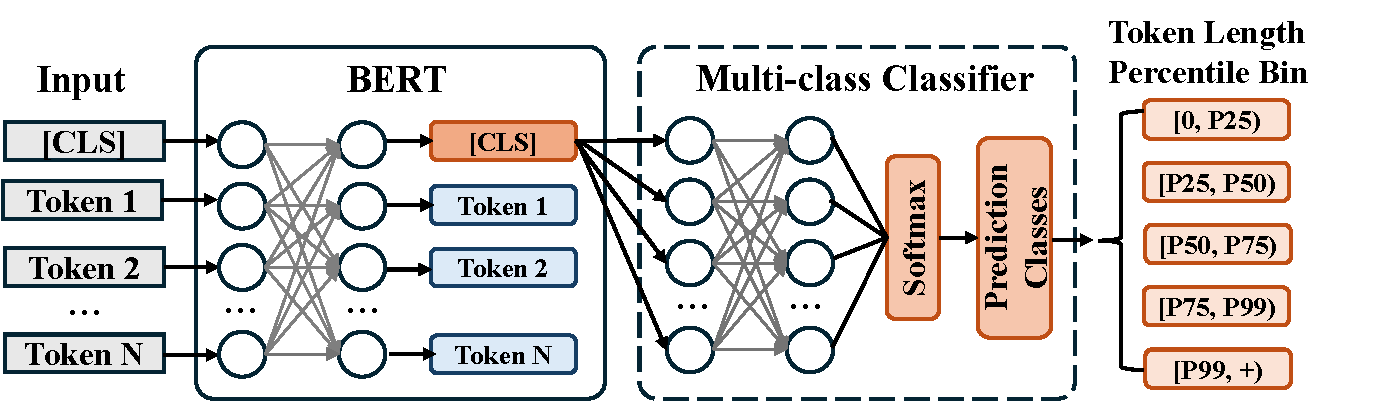
\includegraphics[width=0.95\linewidth]{fig/proxy-model.pdf}
    \caption{Prediction model for output length}
    \label{fig:proxy-model}
    \vspace{-8pt}
\end{figure}

\begin{algorithm}[!t]
\setlength{\textfloatsep}{0.5cm}
\setlength{\floatsep}{0.5cm}
\setlength{\intextsep}{-5em}
\KwData{\textbf{kvUsage}: Predicted kv cache usage map at future sampling points.  \textbf{kvCapacity}: System kv cache capacity. \textbf{futurePoints}:  Step points for future decision-making}
\SetKwFunction{CheckSwitch}{CheckSwitch}
\SetKwProg{Fn}{Function}{:}{}
\SetKwFunction{updateUsage}{UpdateUsage}
\SetKwFunction{schedule}{SchedulePrefill}
\Fn{\CheckSwitch{kvUsage,  kvCapacity}}{
    maxUsage $\gets$ 0 \;
    \ForEach{usage $\in$ kvUsage}{
        \If{usage > maxUsage}{
            maxUsage $\gets$ usage \;
        }
    }
    \If{maxUsage > kvCapacity}{
        Switch to decode\;
    }
    \Else{
        Remain in prefill\;
    }
}
\Fn{\updateUsage{prefillRequest, kvUsage}}{
    inputLen $\gets$ getInputLen(prefillRequest)\;
    predictLen $\gets$ getPredictLen(prefillRequest)\;
    \ForEach{futurePoint $\in$ futurePoints}{
        \If{futurePoint $\leq$ predictLen}{
            kvUsage[futurePoint] += (inputLen + futurePoint)\;
        }
    }
}

\Fn{\schedule{kvUsage,  kvCapacity}}{
    % \tcp{applying continuous batching}
    batch = getPrefillBatch().Launch()\;
    \ForEach{request $\in$ batch}{
        \updateUsage{request, kvUsage}
    }
    \CheckSwitch(kvUsage,  kvCapacity)
}
\caption{Prefill-to-Decode Switch Algorithm}
\label{algo:memusage}
% \vspace{-5pt}
\end{algorithm}

After performing the prefill phase, TD-Pipe requires to determine the timing for switching from prefill to decode.
To reduce the switching frequency between the prefill and decode phase, TD-Pipe tends to execute more prefills before switching to the decode phase.
However, the decode phase also generates KV cache and consumes memory, blindly performing too many prefills will lead to frequent re-computation or offloading in the decode phase, which results in a significant performance drop.
Unfortunately, output lengths are unknown until requests complete and the peak memory usage is also unknown.

To determine how many prefills should be launched without largely exceeding the memory capacity during the decode phase, we propose the AI-based greedy prefill approach.
If we could know input and output lengths of all requests, we could calculate the total memory usage and determine the switching timing.
Furthermore, during the decode phase where all requests progress together, some requests generate new KV cache while others complete, freeing the associated KV cache.
By simulating the memory usage throughout the entire process, we can perform prefills more aggressively. 

To accurately predict the output length for each request, we follow the prediction model introduced in µ-Serve ~\cite{qiu2024muserve}, as illustrated in Figure~\ref{fig:proxy-model}. This model employs a BERT-based multi-class classifier to estimate the output token length for each user request. Specifically, it utilizes the hidden state of the [CLS] token from the final layer of BERT as an aggregate representation of the input, which is then passed through a two-layer feedforward neural network to predict the output length category. These categories are defined as ranges, starting from [P0, P25) to [P99, +), representing the percentage intervals derived from historical inference data. We assume that the inference inputs within a given scenario exhibit strong similarities, allowing us to train the model based on historical patterns. For each request, the predicted output length is assigned based on the average value of the category from the training set. 
Notably, the execution overhead of the prediction model is extremely low and can be neglected during the entire inference process.

With output length predictions, we design a dynamic programming (DP) algorithm, as in Algorithm~\ref{algo:memusage}, to efficiently simulate the memory usage for the subsequent decoding steps after performing new prefills. This simulation is performed after each prefill completes, without introducing significant overhead.
To simplify the computational complexity, we designate certain decode steps in the future for decision-making, referred to as \textit{futurePoints}.
For example, we only check whether the memory usage in the 32nd, 64th, 96th, ..., 992nd, 1024th decode steps exceeds the memory capacity.
After newly launching a batch, the algorithm updates the KV cache usage at these decode steps (\textit{futurePoints}) by checking whether the predicted output lengths exceeds certain decode steps.
With the future KV cache usage, we can determine the timing for switching from prefill to decode by checking whether there exists a \textit{futurePoint} that the memory usage is larger than the memory capacity.

\subsection{Approach-2: Inter-batch Work Stealing}

\begin{figure}[!t]
    \centering    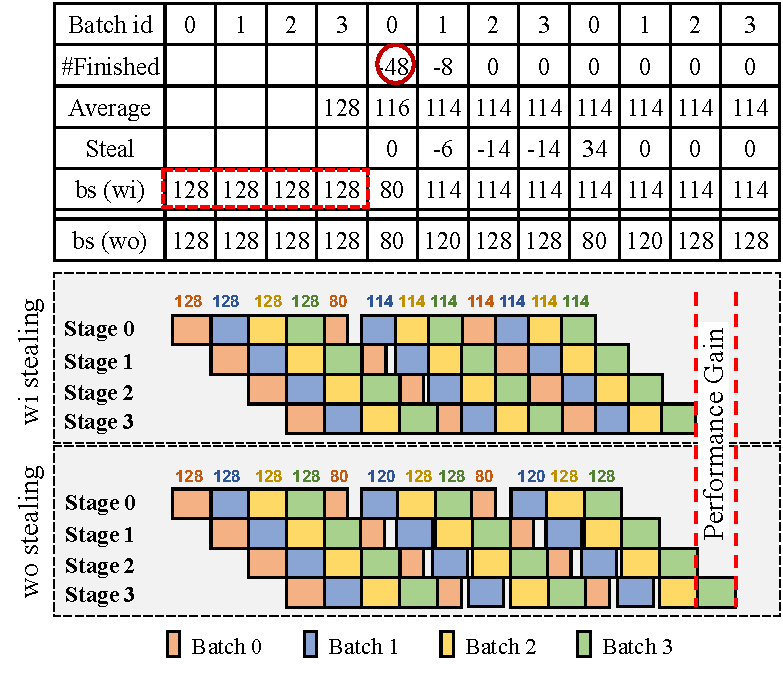
\includegraphics[width=0.95\linewidth]{fig/inter-batch.pdf}
    \caption{The inter-batch work stealing approach. \textbf{bs(wi)} represents the batch size with stealing and \textbf{bs(wo)} represents the batch size without stealing.}
    \label{fig:app-2}
\end{figure}

As the decode phase progresses, requests in different batches complete randomly and the workloads of different batches constantly change, resulting in imbalanced workloads.
Because of data dependencies between decode steps, it can result in pipeline bubbles.
The inter-batch work stealing approach is responsible for ensuring that workloads are evenly distributed across batches throughout the entire decode phase.

Initially, we need to determine when two decode batches can be considered to have equivalent workloads.
The execution time of a single decode step is determined by two factors: batch size and the lengths of KV cache.
The decode phase typically operates on large batch sizes, often in the hundreds, and KV cache lengths also vary significantly across requests.
This huge space makes it hard to accurately compare the execution time between two batches.
To simplify this, we consider batch size as the sole metric for indicating load balance between batches.
This is because linear operations generally dominate execution time in Transformer models across most scenarios and its execution time only relate to batch size.
Moreover, large batch sizes help smooth out execution time fluctuations caused by variation in sequence lengths.

At the beginning, we divide the requests into batches equal to the number of GPUs, with each batch containing the same number of requests.
As the decode phase progresses, requests in different batches complete randomly and the workloads of different batches constantly change, resulting in imbalanced workloads.
To make them balanced, the inter-batch work stealing approach requires to dynamically migrate workloads between batches.
Notably, the batch scheduler can observe the actual batch size of at most one batch at a moment, while other batches remain executing and some requests potentially complete.
Thus, this approach employs the idea of sliding window to balance inter-batch workloads on-the-fly.

When a batch completes and returns, the central scheduler firstly examines the batch and removes the finished requests.
Then, an average batch size is acquired by deducting the number of finished requests from the total number of requests maintained in the sliding window and calculating the average.
The sliding window, with length equal to the number of GPUs, tracks recent batch sizes.
If the current batch contains more requests than the average, the excess requests are temporarily withheld and the batch is submitted for further processing.
And in subsequent iterations, the scheduler will supplement other batches with withheld requests. 
Through this iterative process, the work stealing approach gradually redistributes workloads, effectively mitigating load imbalance. 

Figure~\ref{fig:app-2} demonstrates a slightly extreme example of how this approach gradually achieves load balance in a 4-stage pipeline.  
Initially, 512 requests are evenly divided into four batches of 128. 
After the first iteration, batch 0 completes 48 requests, leaving 80.
As shown in Figure~\ref{fig:app-2}, by applying a sliding window to the last four batches and subtracting the number of completed requests, we obtain an average batch size of 116.
Since the remaining 80 requests in batch 0 are below the current average of 116 requests per batch, all 80 are resubmitted.
8 requests in batch 1 completes and the current average batch size becomes 114. Since the number of requests in batch 1 exceeds 114, the scheduler steals 6 requests from batch 1 and submits only 114. For batch 2 and 3, no requests complete in the first round, and the scheduler similarly steals requests as needed to keep each batch close to the average. In the next iteration, these stolen requests are redistributed to batch 0, thereby achieving balanced workloads across all batches. 
In the lower part of Figure~\ref{fig:app-2}, the imbalanced workloads quickly trend towards balance, and the reduced pipeline bubble translates into performance gains.


\subsection{Approach-3: Spatial-Temporal Intensity Comparison}

\begin{figure}[!t]
    \centering    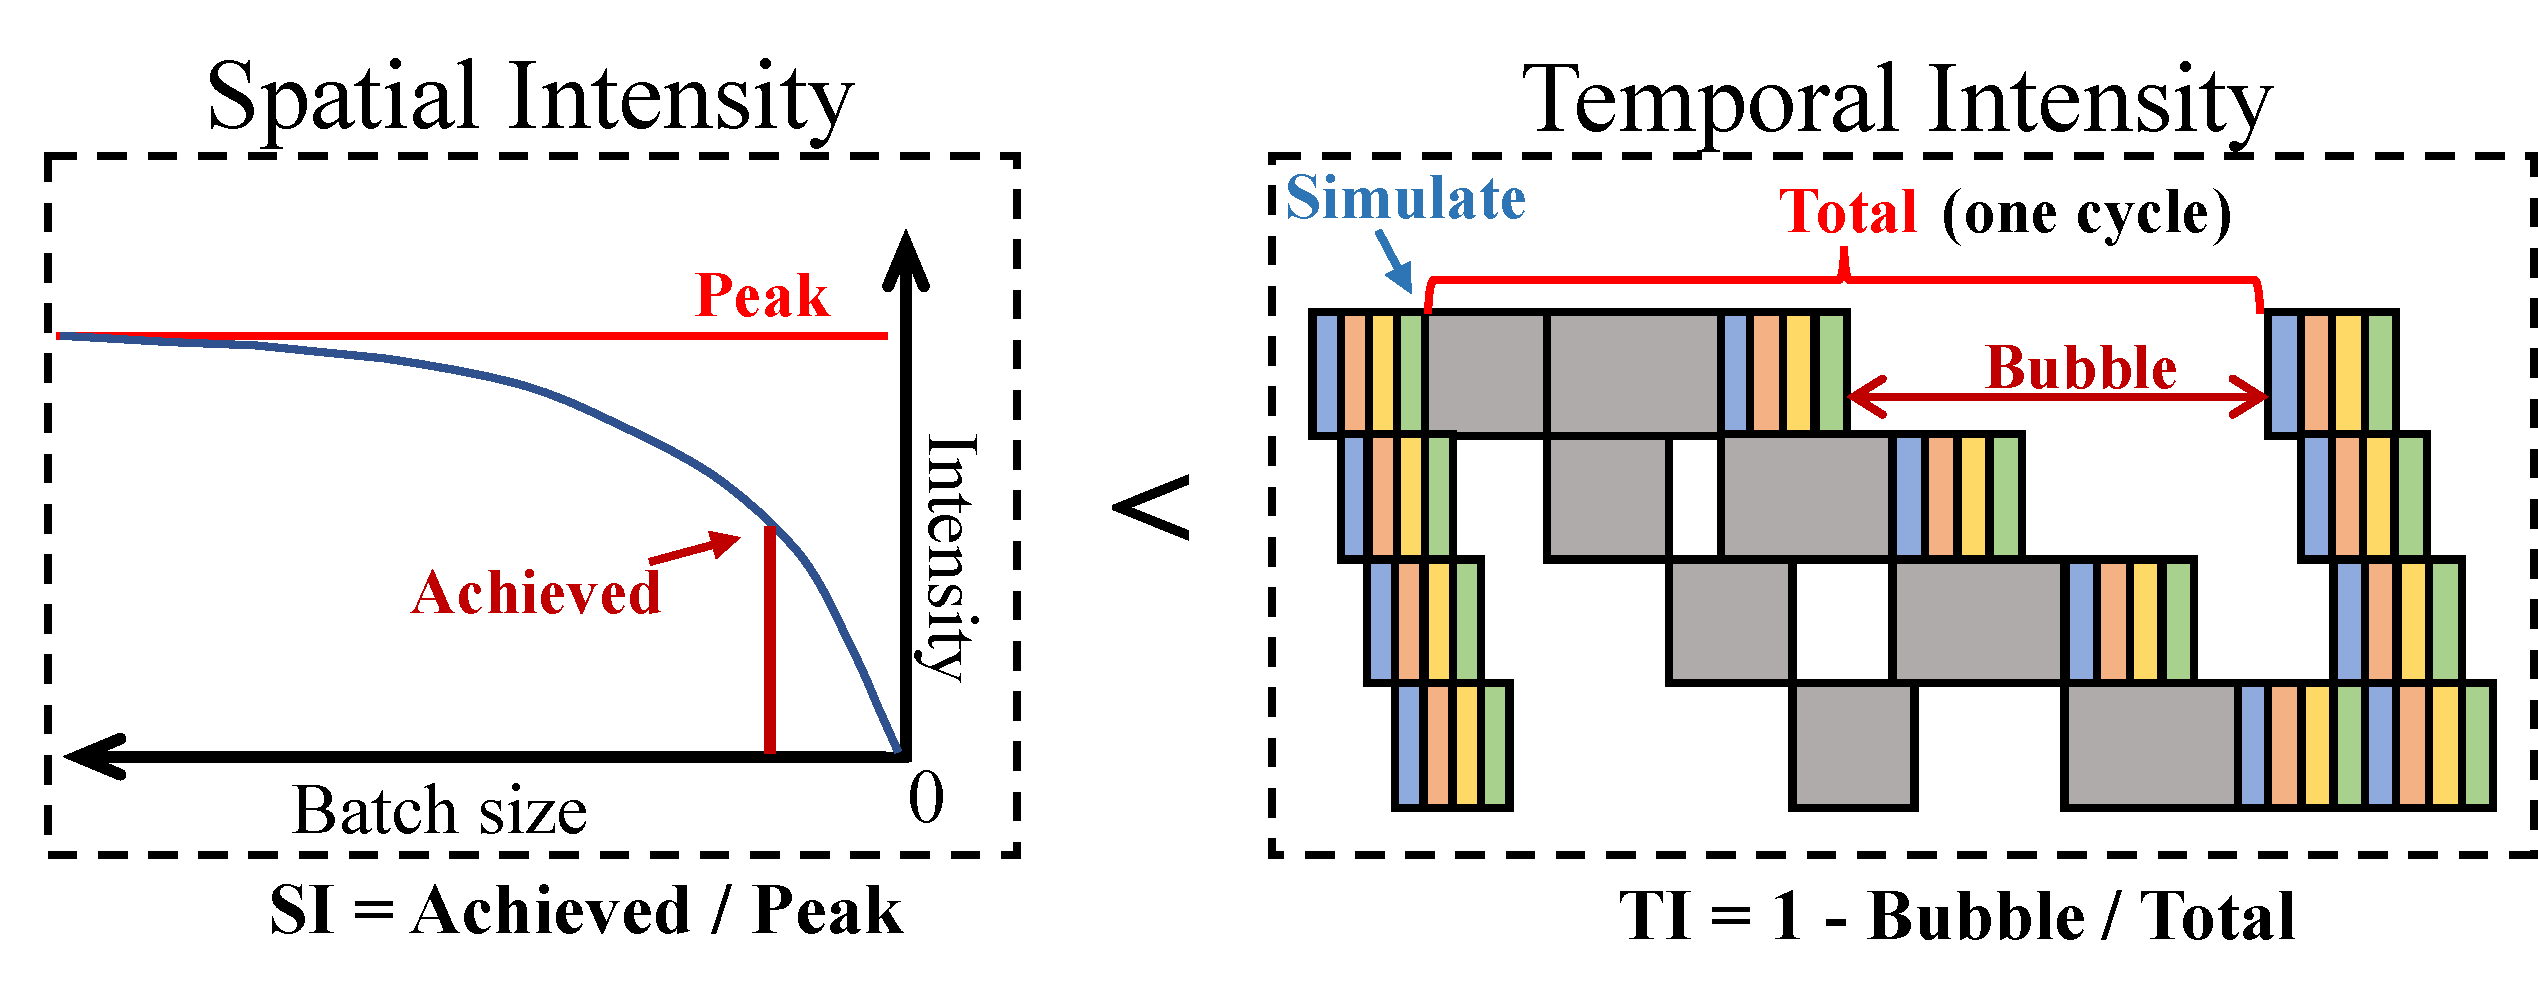
\includegraphics[width=0.95\linewidth]{fig/app-3.pdf}
    \caption{Spatial-temporal intensity comparison approach.}
    \label{fig:app-3}
\end{figure}

In the temporally-disaggregated pipeline architecture, the decode phase acts as the consumer. 
As the decode phase progresses, some requests complete, causing the batch size to decrease and leading to a drop in computational intensity.
If the computational intensity continues to drop, the decode phase would operate in low efficiency. 
However, if we switch to the prefill phase as soon as decode efficiency drops, frequent switching could create bubbles and harm performance.
To handle this dilemma, the spatial-temporal intensity comparison approach aims to determine the optimal timing for switching from decode to prefill.

As illustrated in Figure~\ref{fig:app-3}, the spatial-temporal intensity comparison approach evaluates and compares the computational efficiency of continuing with the decode phase versus switching to the prefill phase. To quantify these two efficiencies, we define spatial intensity for remaining in the decode phase and temporal intensity for switching to the prefill phase.

Spatial intensity is defined as the ratio of the current decode performance to the peak achievable performance.  In detail, we profile the execution time and calculate the average execution time per request using a sufficiently large batch size.
We refer to the reciprocal of the average execution time per request under high computational intensity as the \textit{Peak}. As shown on the left side of Figure~\ref{fig:app-3}, for each batch size, we similarly profile the reciprocal of the average execution time per request, which we denote as \textit{Achieved}. Spatial intensity is then  denoted by:
\vspace{-2pt}
\begin{equation}
\text{Spatial Intensity} = \frac{\textit{Achieved}}{\textit{Peak}}
\end{equation}
Then, temporal intensity is defined as 1 minus the bubble ratio.
The bubble ratio is the proportion of time lost to \textbf{bubble} if a switch occurs now, relative to the duration of the next prefill phase.
As shown in the right side of Figure~\ref{fig:app-3}, for each moment in the decode phase, we calculate the potential \textbf{bubble} and simulate the \textbf{total} time in the next cycle.
For the \textbf{bubble}, it is the difference between the longest prefill and the current decode.
For the \textbf{total} time, it is the accumulation of the pending prefills, each batch's one decode step (can even be ignored), and the bubble.
Since the pending prefills are determined, we can easily calculate their execution time.
Thus, temporal intensity is then denoted by:
\vspace{-2pt}
\begin{equation}
\text{Temporal Intensity} = 1 - \frac{\textit{bubble}}{\textit{total}}
\end{equation}

Based on these two intensities, we design the decision strategy as follows: when the spatial intensity is less than the temporal intensity, the system switches to the prefill phase. Otherwise, it continues with the decode phase.

